
\documentclass[12pt]{article}

\usepackage[utf8]{inputenc}
\usepackage[greek, english]{babel}

% Packages
\usepackage{alphabeta}
\usepackage{amsmath}
\usepackage{amsthm}
\usepackage{caption}
\usepackage{color}
\usepackage{float}
\usepackage{fullpage}
\usepackage{graphicx}
\usepackage{hyperref}
\usepackage{latexsym}
\usepackage{listings}
\usepackage{pxfonts}
\usepackage{stackrel}
\usepackage{subfig}
\usepackage{tikz}
\usepackage{titlesec}

% Commands
\newcommand{\N}{\mathbb{N}}
\newcommand{\R}{\mathbb{R}}
\newcommand{\abs}[1]{\left\lvert#1\right\rvert}
\newcommand{\code}[2]{\lstinputlisting[caption={#2}]{#1}}
\newcommand{\margin}{\hspace{4pt}}
\newcommand{\norm}[1]{\left\lVert#1\right\rVert}

% Environments
\newenvironment{matlab}
	{\begin{figure}[hp]\centering\captionsetup{justification=centering}}
	{\end{figure}}

\newenvironment{rcases}
	{\left.\begin{aligned}}
	{\end{aligned}\right\rbrace}

% Python Syntax Highlighting
\definecolor{string_color}{RGB}{0, 161, 13}
\definecolor{comment_color}{RGB}{46, 46, 46}
\definecolor{keyword_color}{RGB}{0, 112, 191}
\definecolor{background_color}{RGB}{250, 250, 250}

\lstset{
    framesep=15pt,
    xleftmargin=15pt,
    xrightmargin=15pt,
    language=Python,
    captionpos=b,
    numbers=right,
    numberstyle=\small\ttfamily,
    frame=lines,
    showspaces=false,
    showtabs=false,
    breaklines=true,
    showstringspaces=false,
    breakatwhitespace=true,
    commentstyle=\color{comment_color}\textit,
    keywordstyle=\bfseries\color{keyword_color}\textbf,
    stringstyle=\color{string_color}\textit,
    morekeywords={self, lambda, __init__, __del__, __name__, for, in, not, and, or, :},
    basicstyle=\small\ttfamily,
    tabsize=4,
    keepspaces=true,
    columns=flexible,
    backgroundcolor=\color{background_color}
}

% Links
\hypersetup{
    colorlinks=true,
    linkcolor=blue,
    filecolor=magenta,
    urlcolor=cyan,
}

% Lengths
\setlength{\parindent}{0in}
\setlength{\oddsidemargin}{0in}
\setlength{\textwidth}{6.5in}
\setlength{\textheight}{10in}
\setlength{\topmargin}{-1.0in}
\setlength{\headheight}{18pt}

\titlespacing*{\subsection}
{0pt}{5.5ex plus 1ex minus .2ex}{4.3ex plus .2ex}

\title{\hugeΥπολογιστική Γεωμετρία\\Πρώτη Εργασία}
\author{Σιώρος Βασίλειος - 1115201500144\\Ανδρινοπούλου Χριστίνα - 1115201500006}
\date{Μάρτιος 2020}

\begin{document}

\maketitle

\pagenumbering{gobble}

\pagebreak


\subsection*{1. Implement an algorithm that takes as input three points in the plane. checks
    that they form a triangle and whether the interior of the triangle contains the origin (0, 0) or
    not.}

\vspace{2in}

\pagebreak

\subsection*{2. Given a circle of radius r in the plane with (0, 0) as center, implement an
    algorithm that finds the total lattice points on the circumference. Lattice Points are points
    with integer coordinates.}

\vspace{2in}

\subsubsection*{Thought Process}

Σε ένα καρτεσιανό σύστημα συντεταγμένων, ένας κύκλος με κέντρο το σημείο (a, b)
και ακτίνα r είναι ένα σχήμα το οποίο αποτελείται από όλα τα σημεία των οποίων
οι συντεταγμένες ικανοποιούν την παρακάτω εξίσωση. \\

\[ (x - a) ^ 2 + (y - b) ^ 2 = r ^ 2 \]

Αν ο κύκλος έχει ως κέντρο την αρχή των αξόνων, δηλαδή το σημείο \( (0, 0) \), τότε
η παραπάνω εξίσωση παίρνει την παρακάτω απλούστερη μορφή. \\

\[ x ^ 2 + y ^ 2 = r ^ 2 \]

Τα σημεία πλέγματος, επί της περιφέρειας ενός κύκλου, είναι τα σημεία που ανήκουν
στην περιφέρεια του και έχουν ακέραιες συντεταγμένες. \\

The lattice points on the circumference of a circle, are the points along the circumference that have integer coordinates.

Any point whose euclidean distance to the center of the circle is greater than the radius of the circle does not belong to the circle.

Thus, if the circle is centred at the origin `(0, 0)`, any point whose x or y coordinate' s absolute value is greater than the radius of the circle does not belong to the circle.

Hence, the lattice points are a subset of the set of points which have as x and y coordinates, integer values in the range `[-radius, +radius]`.

For example, for a circle with a radius of 1 we only need to check the points

\subsubsection*{Running the code}

\begin{matlab}
    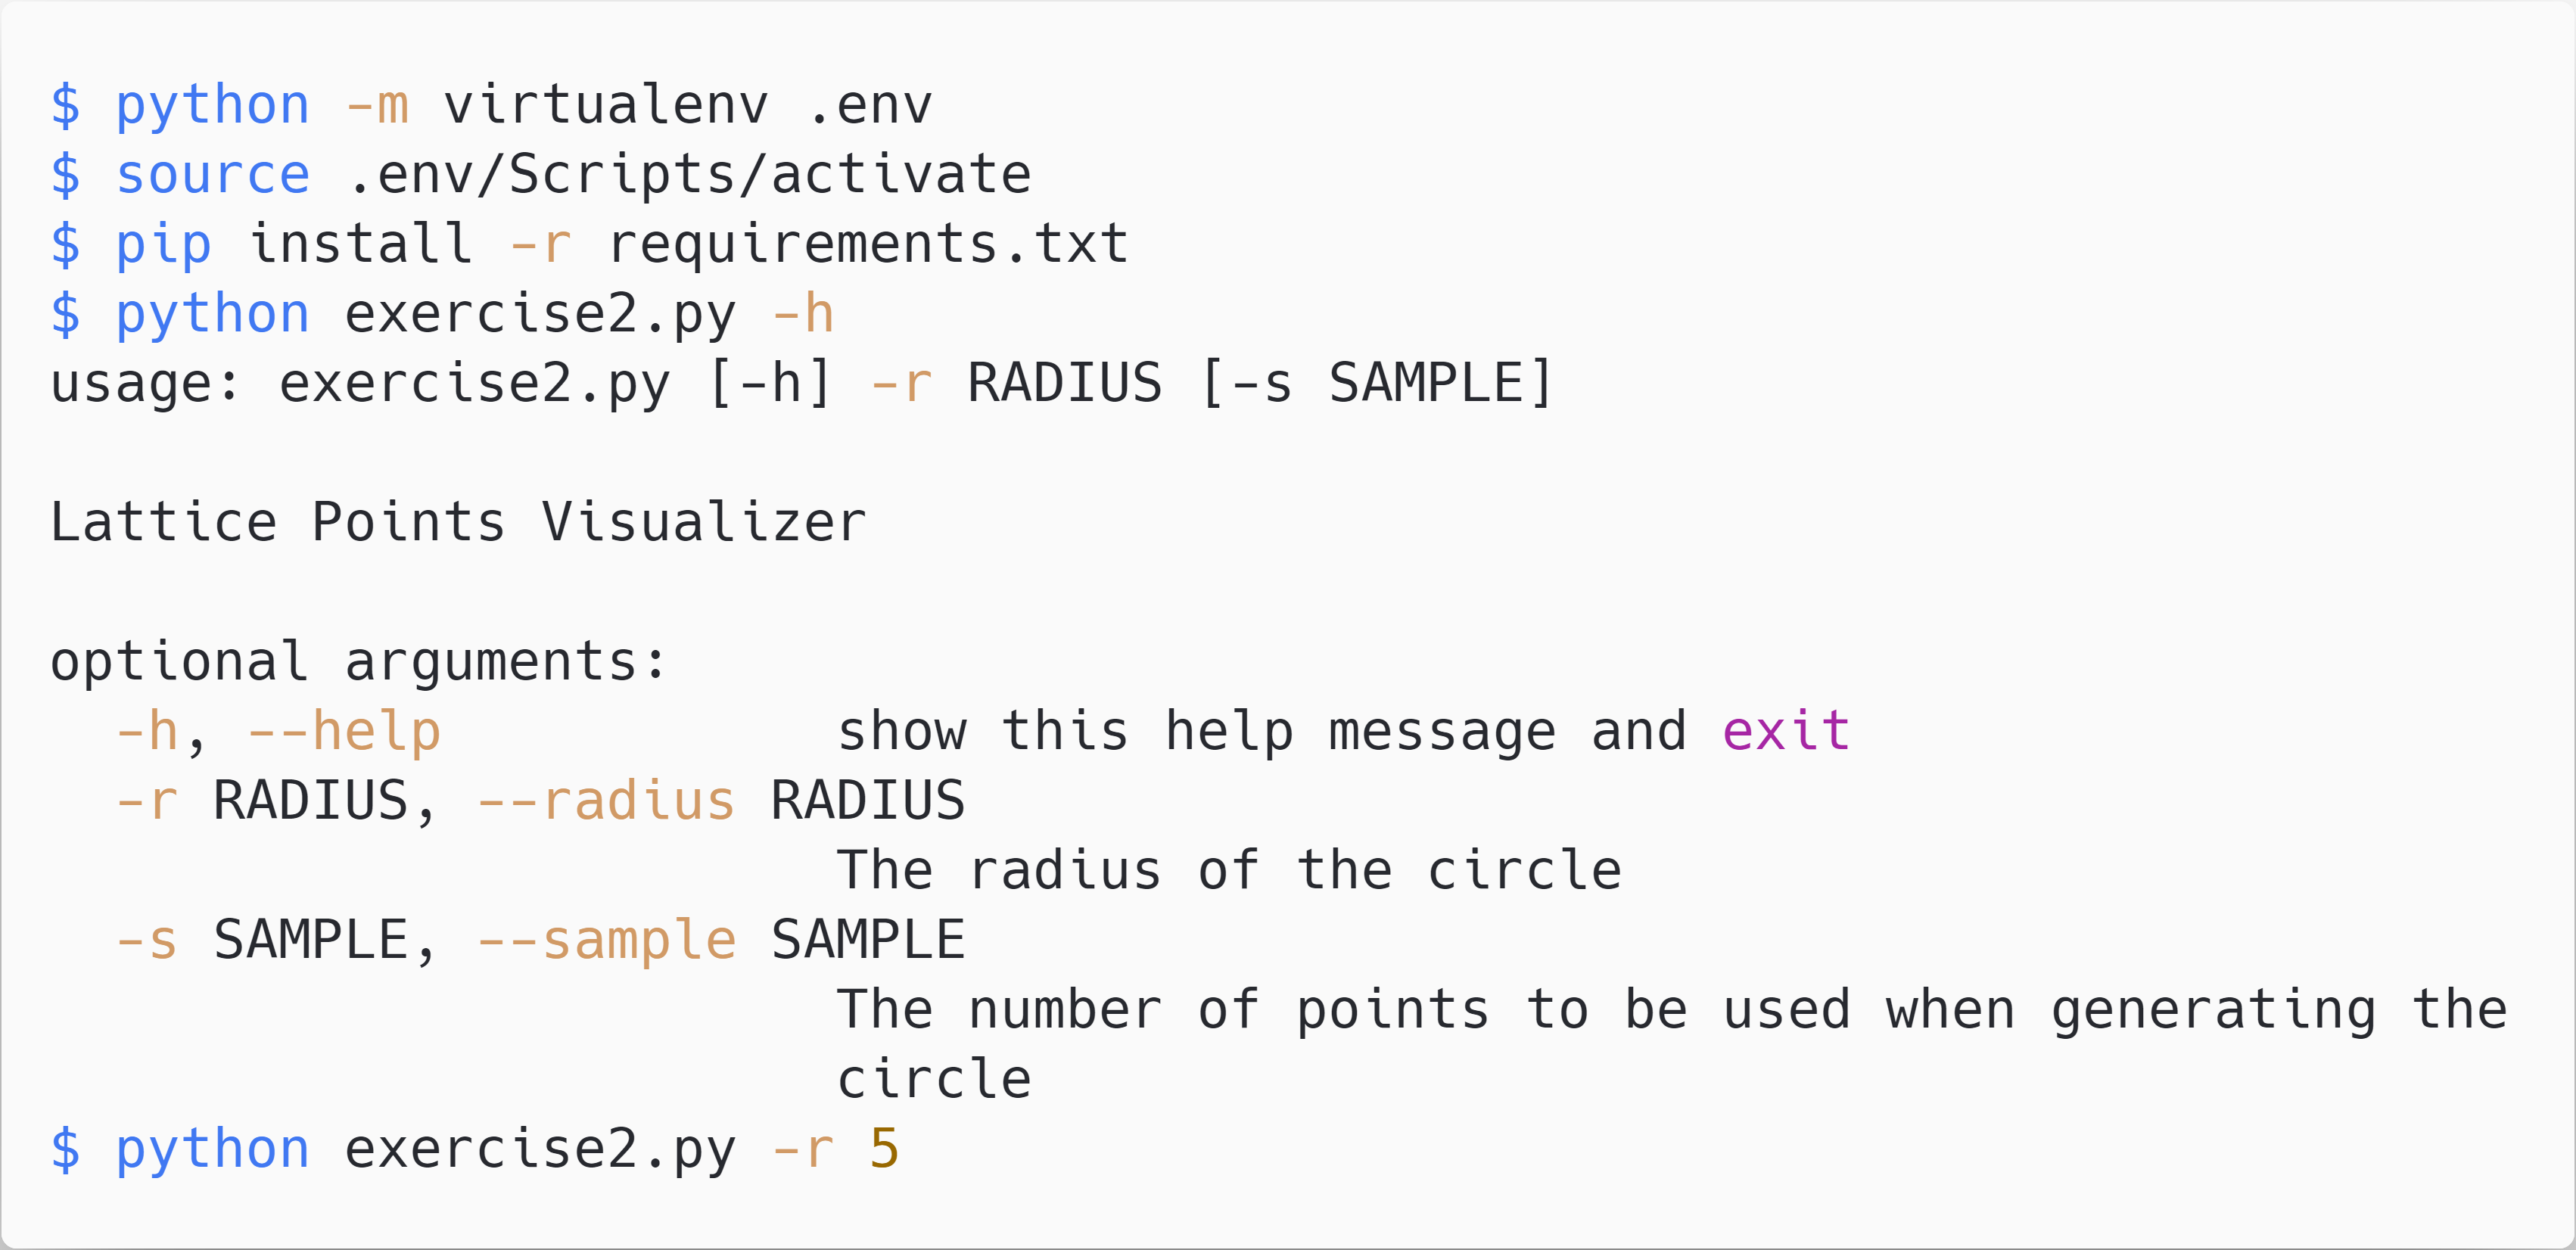
\includegraphics[scale=0.140]{images/exercise2.png}
\end{matlab}

\pagebreak

\subsection*{3. Implement the incremental 2D algorithm for computing the convex hull of a
    finite set of points in the plane.}

\vspace{2in}

\pagebreak

\subsection*{4. Implement the gift wrap algorithm for computing the convex hull of a finite
    set of points in the plane .}

\vspace{2in}

\subsubsection*{Running the code}

\begin{matlab}
    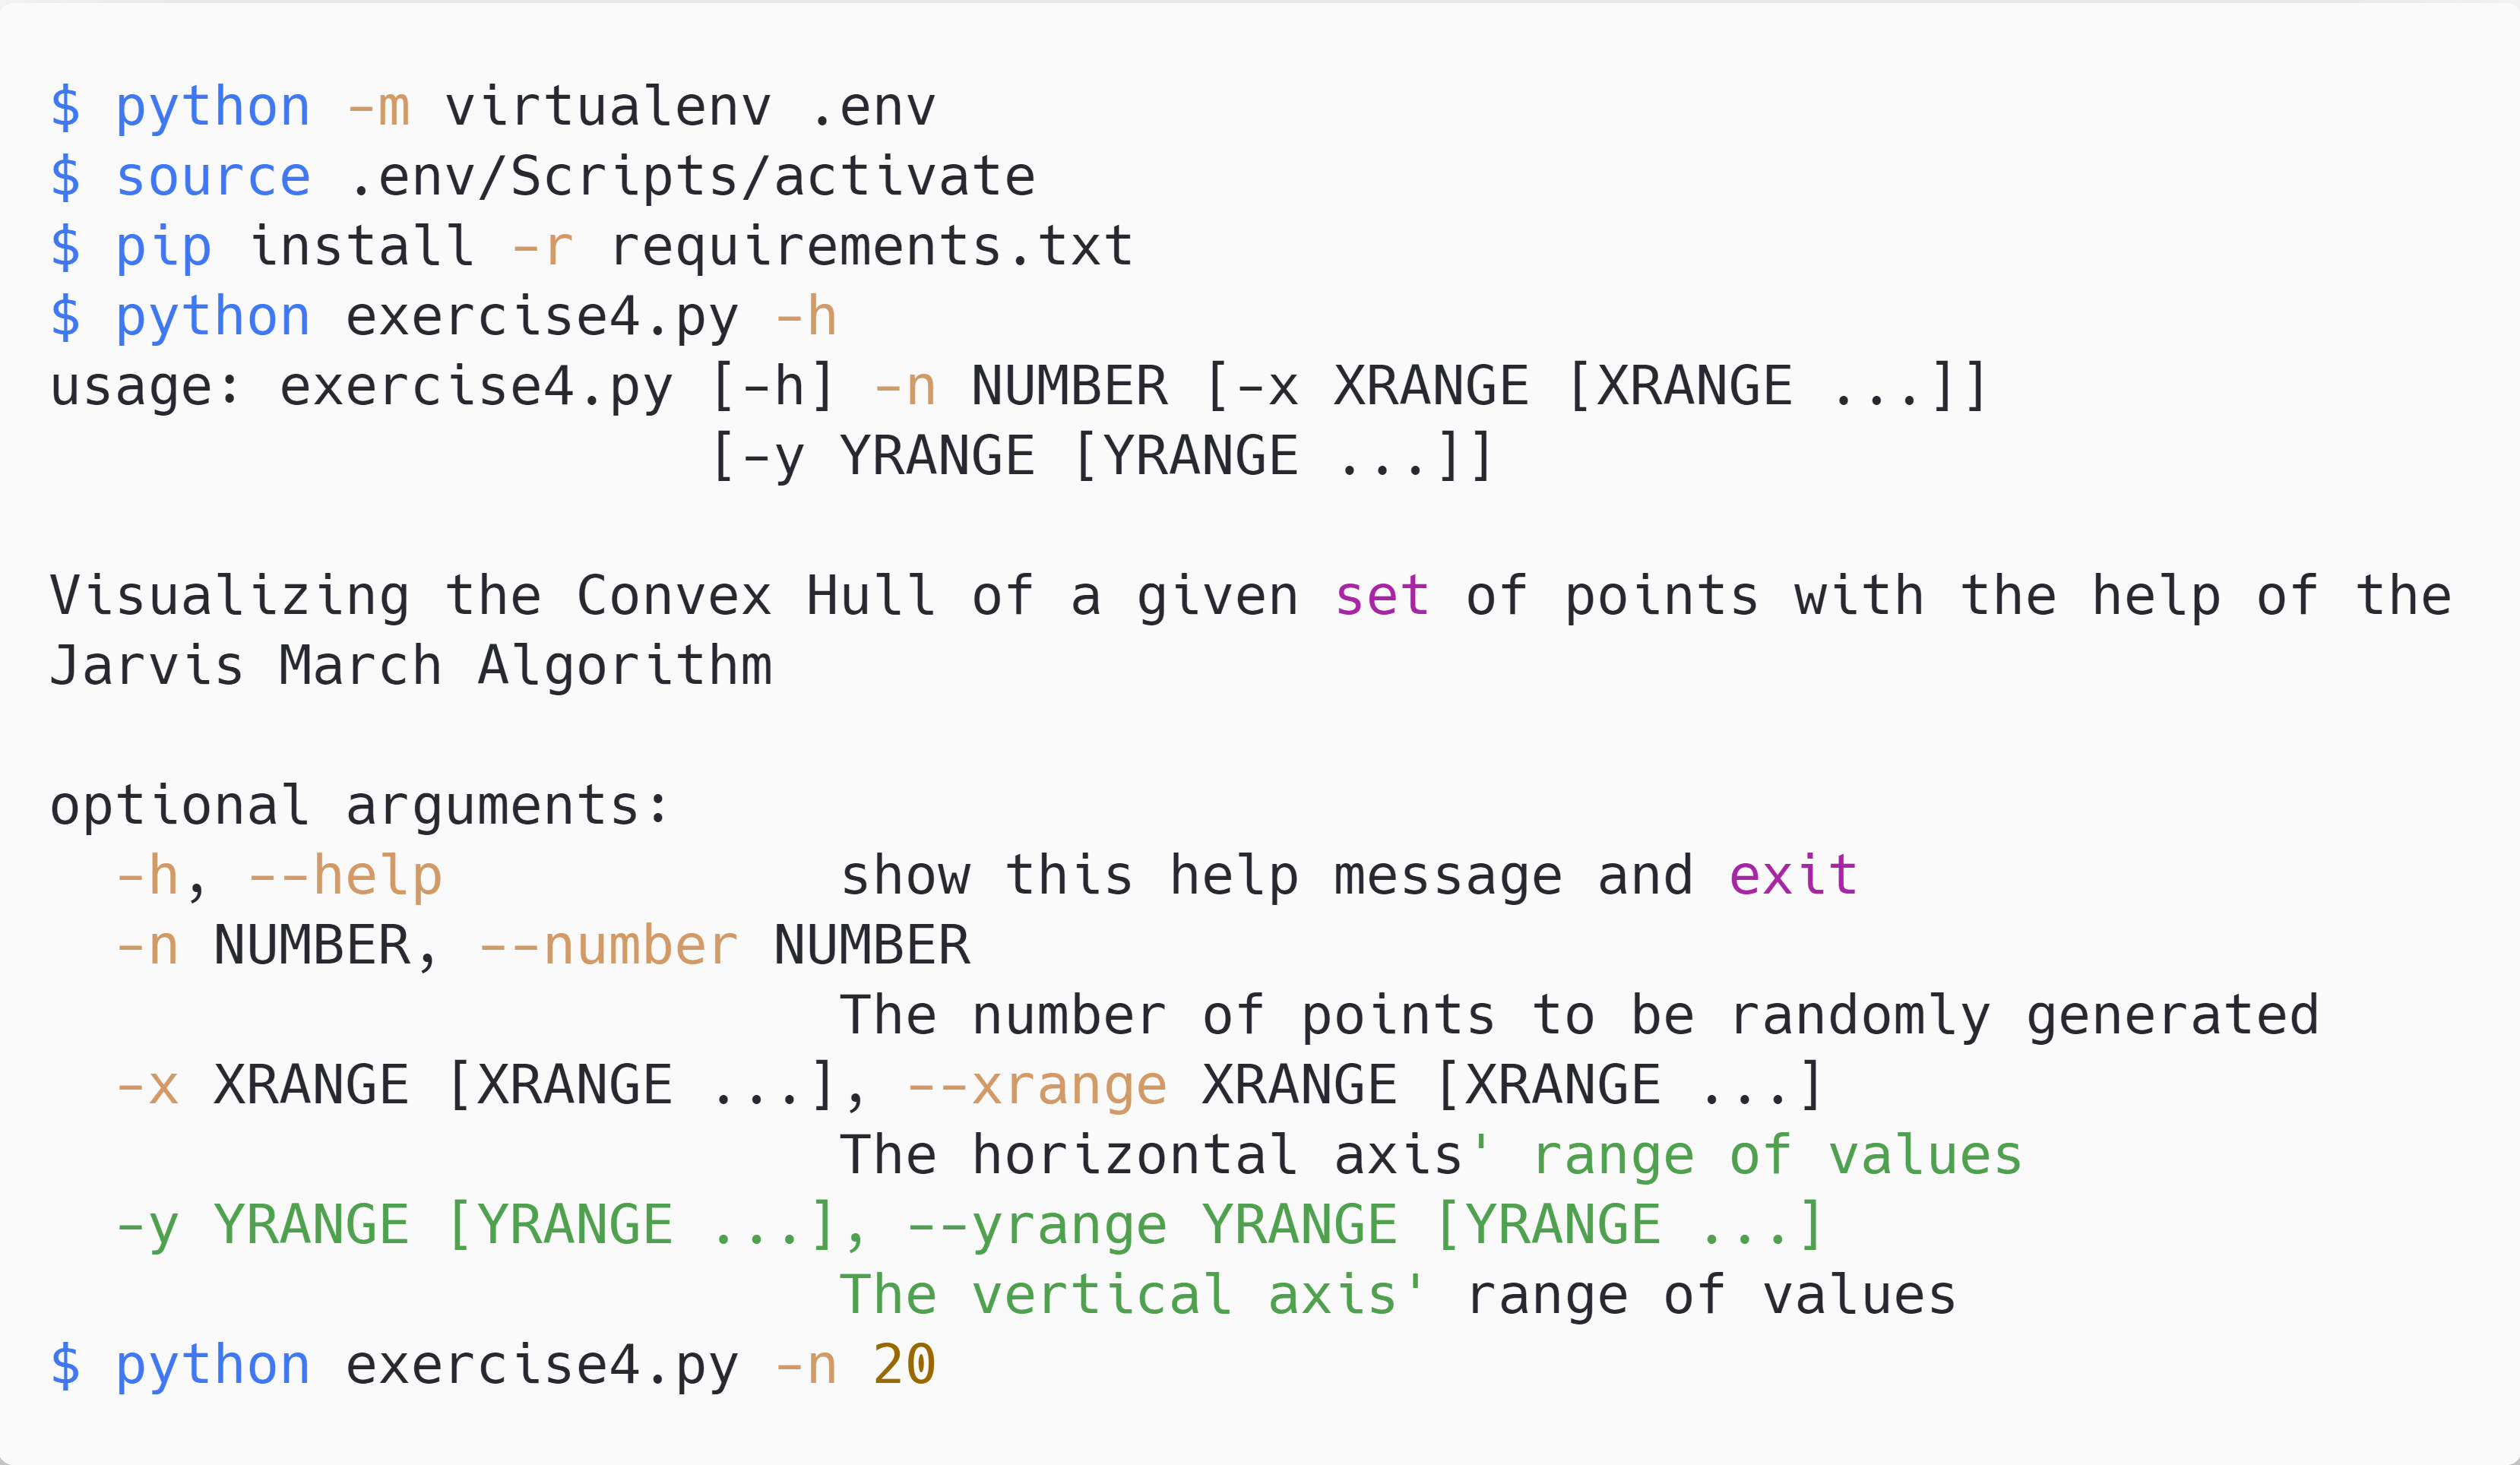
\includegraphics[scale=0.140]{images/exercise4.png}
\end{matlab}

\pagebreak

\end{document}
